\documentclass[12pt,a4paper]{report}

\usepackage[utf8]{inputenc}
\usepackage[T1]{fontenc}
\usepackage{mathptmx} % Times New Roman
\usepackage[left=1.5in,right=1.0in,top=1.0in,bottom=1.0in]{geometry}
\usepackage{setspace}
\onehalfspacing

\usepackage{graphicx}
\usepackage{fancyhdr}
\usepackage{titlesec}
\usepackage{amsmath}
\usepackage{tabularx}
\usepackage{booktabs}
\usepackage{array}
\usepackage{longtable}
\usepackage{caption}
\usepackage{enumitem}
\usepackage{float}
\usepackage{microtype}
\usepackage[hidelinks]{hyperref}

% Break long URLs and monospace identifiers cleanly
\usepackage{url}
\def\UrlBreaks{\do\/\do-\do_}

% Page numbering and header styling
\pagestyle{fancy}
\fancyhf{}
\fancyhead[R]{\nouppercase{\leftmark}}
\fancyfoot[C]{\thepage}
\renewcommand{\headrulewidth}{0.5pt}
\renewcommand{\footrulewidth}{0pt}
\setlength{\headheight}{15pt}

% Caption styling: academic 10.5pt bold title with standard font
\captionsetup{
  font={small,stretch=1.2},
  labelfont=bf,
  justification=centering,
  skip=8pt
}

% Chapter and section title formatting
\titleformat{\chapter}[display]
  {\normalfont\bfseries\centering}{\Large CHAPTER \thechapter}{8pt}{\LARGE\uppercase}
\titlespacing*{\chapter}{0pt}{-10pt}{20pt}

\titleformat{\section}
  {\normalfont\bfseries\large}{\thesection}{1em}{}
\titlespacing*{\section}{0pt}{14pt}{6pt}

\titleformat{\subsection}
  {\normalfont\bfseries\normalsize}{\thesubsection}{1em}{}
\titlespacing*{\subsection}{0pt}{10pt}{4pt}

% Table column helper definitions
\newcolumntype{L}[1]{>{\raggedright\arraybackslash}p{#1}}
\newcolumntype{C}[1]{>{\centering\arraybackslash}p{#1}}
\newcolumntype{Y}{>{\raggedright\arraybackslash}X}

\begin{document}

% -------------------------------------------------------------
% COVER / TITLE PAGE (Unnumbered)
% -------------------------------------------------------------
\begin{titlepage}
\thispagestyle{empty}
\begin{center}
    \vspace*{0.2cm}
    {\large \textbf{ORIGINCHAIN: BLOCKCHAIN-BASED QUALITY ASSURANCE,\\
    AUTHENTICATION AND SUPPLY-CHAIN TRACEABILITY\\
    FOR LUXURY COSMETICS}\par}
    
    \vspace{1.0cm}
    {\normalsize Submitted in partial fulfilment of the requirements of the degree of\par}
    \vspace{0.3cm}
    {\large \textbf{BACHELOR OF COMPUTER ENGINEERING}\par}
    
    \vspace{0.8cm}
    {\normalsize by\par}
    \vspace{0.3cm}
    {\textbf{Durva Waghchaure (23102152)}\par}
    \vspace{0.15cm}
    {\textbf{Aryan Singh (23102154)}\par}
    \vspace{0.15cm}
    {\textbf{Purvika Thombare (23102097)}\par}
    \vspace{0.15cm}
    {\textbf{Aradhya Thakur (23102110)}\par}
    
    \vspace{0.9cm}
    {\normalsize Under the Guidance of\par}
    \vspace{0.25cm}
    {\large \textbf{Prof. Pranali Patil}\par}
    
    \vfill
    
\includegraphics[width=2.6cm]{images/college_logo.png}\par
    \vspace{0.35cm}
    {\large \textbf{Department of Computer Engineering}\par}
    \vspace{0.15cm}
    {\large \textbf{A. P. SHAH INSTITUTE OF TECHNOLOGY, THANE}\par}
    \vspace{0.15cm}
    {\normalsize \textbf{University of Mumbai}\par}
    \vspace{0.15cm}
    {\normalsize \textbf{2026--2027}\par}
\end{center}
\end{titlepage}

\pagenumbering{roman}
\setcounter{page}{2}

% -------------------------------------------------------------
% CERTIFICATE (Page ii)
% -------------------------------------------------------------
\newpage
\thispagestyle{plain}
\begin{center}
    
\includegraphics[width=2.2cm]{images/college_logo.png}\par
    \vspace{0.25cm}
    {\large \textbf{A. P. SHAH INSTITUTE OF TECHNOLOGY, THANE}\par}
    \vspace{0.45cm}
    {\Large \textbf{CERTIFICATE}\par}
\end{center}
\vspace{0.5cm}
\noindent This is to certify that the project entitled \textbf{``OriginChain: Blockchain-Based Quality Assurance, Authentication and Supply-Chain Traceability for Luxury Cosmetics''} is a bonafide work of \textbf{Durva Waghchaure (23102152)}, \textbf{Aryan Singh (23102154)}, \textbf{Purvika Thombare (23102097)}, and \textbf{Aradhya Thakur (23102110)} submitted to the University of Mumbai in partial fulfilment of the requirement for the award of the degree of \textbf{Bachelor of Engineering in Computer Engineering}.

\vspace{2.2cm}
\noindent
\begin{tabular*}{\textwidth}{@{\extracolsep{\fill}}cc}
    \underline{\hspace{5.2cm}} & \underline{\hspace{5.2cm}} \\
    \textbf{Prof. Pranali Patil} & \textbf{Dr. Rushikesh R. Nikam} \\
    Guide & Project Coordinator \\
    \vspace{2.0cm} & \vspace{2.0cm} \\
    \underline{\hspace{5.2cm}} & \underline{\hspace{5.2cm}} \\
    \textbf{Dr. Sachin Malave} & \textbf{Dr. Uttam Kolekar} \\
    Head of Department & Principal \\
\end{tabular*}

\vspace{0.8cm}
\noindent Date: \underline{\hspace{3.5cm}}

% -------------------------------------------------------------
% PROJECT APPROVAL (Page iii)
% -------------------------------------------------------------
\newpage
\thispagestyle{plain}
\begin{center}
    
\includegraphics[width=2.2cm]{images/college_logo.png}\par
    \vspace{0.25cm}
    {\large \textbf{A. P. SHAH INSTITUTE OF TECHNOLOGY, THANE}\par}
    \vspace{0.45cm}
    {\Large \textbf{Project Report Approval for B.E.}\par}
\end{center}
\vspace{0.5cm}
\noindent This project report entitled \textbf{``OriginChain: Blockchain-Based Quality Assurance, Authentication and Supply-Chain Traceability for Luxury Cosmetics''} by \textbf{Durva Waghchaure, Aryan Singh, Purvika Thombare, and Aradhya Thakur} is approved for the degree of \textbf{Bachelor of Engineering in Computer Engineering, 2026--2027}.

\vspace{2.0cm}
\noindent \textbf{Examiners:}

\vspace{0.8cm}
\noindent
\begin{tabular*}{\textwidth}{@{\extracolsep{\fill}}ll}
    \textbf{Examiner Name} & \textbf{Signature} \\[1.6cm]
    1. \underline{\hspace{6.5cm}} & \underline{\hspace{5.5cm}} \\[1.6cm]
    2. \underline{\hspace{6.5cm}} & \underline{\hspace{5.5cm}} \\
\end{tabular*}

\vspace{2.0cm}
\noindent Date: \underline{\hspace{4cm}} \hfill Place: \underline{\hspace{4cm}}

% -------------------------------------------------------------
% DECLARATION (Page iv)
% -------------------------------------------------------------
\newpage
\thispagestyle{plain}
\begin{center}
    {\Large \textbf{Declaration}\par}
\end{center}
\vspace{0.6cm}
\noindent We declare that this written submission represents our ideas in our own words and where others' ideas or words have been included, we have adequately cited and referenced the original sources. We also declare that we have adhered to all principles of academic honesty and integrity and have not misrepresented or fabricated or falsified any idea/data/fact/source in our submission. We understand that any violation of the above will be cause for disciplinary action by the Institute and can also evoke penal action from the sources which have thus not been properly cited or from whom proper permission has not been taken when needed.

\vspace{2.0cm}
\noindent
\begin{tabular*}{\textwidth}{@{\extracolsep{\fill}}lr}
    \underline{\hspace{5.5cm}} & \underline{\hspace{5.5cm}} \\
    \textbf{Durva Waghchaure (23102152)} & \textbf{Aryan Singh (23102154)} \\[2.0cm]
    \underline{\hspace{5.5cm}} & \underline{\hspace{5.5cm}} \\
    \textbf{Purvika Thombare (23102097)} & \textbf{Aradhya Thakur (23102110)} \\
\end{tabular*}

\vspace{1.8cm}
\noindent Date: \underline{\hspace{3.5cm}}

% -------------------------------------------------------------
% ABSTRACT (Page v - Single page, perfectly fitted)
% -------------------------------------------------------------
\newpage
\thispagestyle{plain}
\begin{center}
    {\Large \textbf{Abstract}\par}
\end{center}
\vspace{0.25cm}
{\small\setstretch{1.12}
Counterfeit and mishandled luxury cosmetics are difficult for a buyer to detect: a bottle may look perfect while its contents, batch history or storage conditions differ from what the label claims. Static barcodes and printed seals are easy to copy, and a conventional database can be edited by anyone with enough privilege. This project, \textbf{OriginChain}, proposes and demonstrates a blockchain-based system that combines stage-by-stage quality assurance with tamper-evident product authentication and traceability for luxury cosmetics.

The implemented demonstration follows one fictional flagship product, the Aurelia Prestige Renewal Serum, from raw-material receipt through manufacturing, distribution and retail to consumer verification. Each actor (supplier, manufacturer, distributor, retailer) must pass a defined set of quality checks, with supporting PDF/PNG/JPEG evidence, before custody can move on. Evidence files are hashed with Keccak-256; compact fingerprints of the product, of each approved stage and of each evidence file are committed to a Solidity smart contract running on a local Hardhat Ethereum Virtual Machine. Full operational records stay off-chain in SQLite, so the ledger remains small and private. The backend is built with FastAPI and Web3.py; users authenticate with Argon2-hashed passwords and short-lived JSON Web Tokens, and role-based access control is enforced on the server and again by the contract's owner checks.

A consumer can enter a product code and receive a redacted, read-only verification result that reports whether the product is Authentic or Suspicious, whether every stage was approved, and which evidence the manufacturer chose to make public. A built-in tamper demonstration shows that editing a database record is detected because the recomputed metadata hash no longer matches the on-chain value. Quality gates are mapped to metadata of real standards (the Cosmetics Rules 2020 and selected BIS and ISO cosmetics standards) purely as traceability references; the project makes no certification or compliance claim. The current build passes 51 backend tests and 17 smart-contract tests.

\vspace{0.25cm}
\noindent \textbf{Contribution to Sustainable Development Goals (SDGs):} OriginChain supports SDG 12 (Responsible Consumption and Production) by making product origin and handling transparent and by discouraging counterfeit goods; SDG 9 (Industry, Innovation and Infrastructure) through an innovative, auditable digital infrastructure for supply chains; SDG 3 (Good Health and Well-being) by reducing the chance that unsafe or substandard cosmetics reach users; and SDG 16 (Peace, Justice and Strong Institutions) through accountable, attributable and tamper-evident records.

\vspace{0.25cm}
\noindent \textbf{Layout of the Report:} The first chapter introduces the problem and the project. The second reviews the literature on blockchain traceability, anti-counterfeiting and cosmetics quality standards. The third states the limitations of existing systems and the research gap, and the fourth gives the problem statement, objectives and scope. The fifth presents the proposed system with its architecture and UML diagrams, algorithms, design details and methodology. The sixth describes the experimental setup, the seventh the project plan, the eighth the expected outcome and the ninth the projected cost analysis, followed by references.
\par}

% -------------------------------------------------------------
% TABLE OF CONTENTS (Page vi)
% -------------------------------------------------------------
\newpage
\tableofcontents

% -------------------------------------------------------------
% LIST OF FIGURES & LIST OF TABLES (Page vii)
% -------------------------------------------------------------
\newpage
\listoffigures
\vspace{0.8cm}
\listoftables

% -------------------------------------------------------------
% ABBREVIATIONS (Page viii)
% -------------------------------------------------------------
\newpage
\thispagestyle{plain}
\begin{center}
    {\Large \textbf{ABBREVIATIONS}\par}
\end{center}
\vspace{0.4cm}
\noindent
\begin{table}[H]
\centering
\renewcommand{\arraystretch}{1.12}
\begin{tabularx}{\textwidth}{p{3.2cm} Y}
\toprule
\textbf{Abbreviation} & \textbf{Expansion} \\
\midrule
ABI & Application Binary Interface \\
API & Application Programming Interface \\
BIS & Bureau of Indian Standards \\
CoA & Certificate of Analysis \\
DApp & Decentralized Application \\
DFD & Data Flow Diagram \\
EVM & Ethereum Virtual Machine \\
GMP & Good Manufacturing Practice \\
IPFS & InterPlanetary File System \\
ISO & International Organization for Standardization \\
JWT & JSON Web Token \\
NFC & Near Field Communication \\
OECD & Organisation for Economic Co-operation and Development \\
PET & Preservative Efficacy Testing \\
QR & Quick Response \\
RBAC & Role-Based Access Control \\
RFID & Radio-Frequency Identification \\
SDG & Sustainable Development Goals \\
UML & Unified Modeling Language \\
\bottomrule
\end{tabularx}
\end{table}

\newpage
\pagenumbering{arabic}
\setcounter{page}{1}

% -------------------------------------------------------------
% CHAPTER 1: INTRODUCTION
% -------------------------------------------------------------
\chapter{Introduction}

\section{Background and Motivation}
Counterfeiting is a large and growing problem in global trade. An OECD and EUIPO study estimated that counterfeit and pirated goods made up roughly 3.3 percent of world trade in 2016 [1]. Luxury cosmetics are particularly exposed: they carry a high price, are easy to refill or re-label, and a buyer cannot judge a sealed bottle's authenticity by its appearance. Unlike a counterfeit handbag, a counterfeit serum is applied to the skin, so contamination, wrong ingredients or poor storage can cause irritation or infection. Consumers, brands and regulators therefore need a trustworthy way to confirm that a product is genuine and was handled correctly.

Printed barcodes, holograms and static QR codes can be duplicated, and centralised databases depend on a single operator, so a privileged insider can silently alter a record. Blockchain offers a different trust model: an append-only ledger whose blocks are linked by cryptographic hashes, so altering an old entry invalidates every later block [2], [3]. Smart contracts on platforms such as Ethereum enforce rules without a trusted intermediary [4], [5], making blockchain a strong foundation for traceability, provided that large and sensitive data stay off the chain [6]. We therefore asked what a luxury-cosmetics supply chain really needs: proof that each party passed meaningful quality checks, tamper-proof evidence, controlled access for each role, and a consumer view that builds trust without leaking internal information.

\vspace{0.3cm}
\noindent \textbf{Sustainable Development Goals:} OriginChain supports SDG 3 (Good Health and Well-being) by reducing the chance that counterfeit cosmetics reach consumers, SDG 9 (Industry, Innovation and Infrastructure) through auditable blockchain-based infrastructure, SDG 12 (Responsible Consumption and Production) through transparent product origin, and SDG 16 (Peace, Justice and Strong Institutions) through tamper-evident records.

\vspace{0.3cm}
\noindent \textbf{Program Outcomes:} PO1 and PO2 are met through engineering fundamentals and the literature survey, PO3 through the system design, PO5 through tools such as FastAPI, Solidity and Hardhat, PO6 and PO7 through consumer safety and societal impact, PO9 and PO10 through teamwork, this report and the demonstration, and PO11 through project planning and cost analysis.

\vspace{0.3cm}
\noindent \textbf{Program Specific Outcomes:} PSO1 is met by building a complete working application, PSO2 by following standard software practices with 68 automated tests, and PSO3 by using modern blockchain technology that can lead to entrepreneurship, higher studies or industry work.

\section{Overview of OriginChain}
OriginChain is a working, end-to-end demonstration that tracks one fictional luxury anti-aging serum, the Aurelia Prestige Renewal Serum (product code \texttt{OC\allowbreak-LUX\allowbreak-SERUM\allowbreak-0001}, batch \texttt{APR\allowbreak-2026\allowbreak-001}), from raw-material receipt to the retail shelf. The product, the companies and all inspection results are fictional demonstration data; only the standards metadata that the quality checks refer to is real. The system is built around four core ideas:
\begin{itemize}[leftmargin=1.8em, itemsep=3pt, parsep=0pt]
    \item \textbf{Stage-gated quality assurance:} The supply chain is modelled as four operational stages: raw-material supplier, manufacturer, distributor and retailer. Each stage has a defined list of quality checks (24 in total: 5 supplier, 8 manufacturer, 5 distributor and 6 retail). A stage can be approved, and custody can be transferred, only when every mandatory check passes and every required piece of evidence exists and is intact.
    \item \textbf{Evidence with integrity and trust:} Certificates, laboratory reports and inspection photographs are uploaded as PDF, PNG or JPEG files, hashed with Keccak-256, and re-verified on demand. For critical reports (certificate of analysis, microbiology and preservation efficacy) the issuer must also be currently trusted in a local registry of fictional issuers.
    \item \textbf{Details off-chain, fingerprints on-chain:} Full records and files remain in SQLite and on disk. The Solidity contract stores only 32-byte hashes, owner addresses, status codes and events, which keeps the ledger compact and private while still making tampering detectable.
    \item \textbf{Consumer verification:} Anyone can enter a product code and receive a redacted result: Authentic or Suspicious, the four-stage quality journey, provenance by role, and any evidence explicitly marked public. Internal notes, files and identifiers are never exposed.
\end{itemize}

Behind these ideas sit a FastAPI backend with role-based access control, an audit log of every meaningful action, a single-page web interface that adapts to the signed-in role, and a set of automated tests. A built-in tamper demonstration lets an administrator edit a stored record and then shows the consumer view turning from Authentic to Suspicious, which makes the value of the on-chain fingerprint visible in a presentation.

\section{Why Luxury Cosmetics}
Cosmetics are an ideal test case for a quality-aware traceability system for three reasons. First, they combine high commercial value with direct human safety sensitivity, so both product authenticity and custody handling matter. Second, a finished cosmetic depends on several upstream parties (ingredient suppliers, contract or in-house manufacturers, distribution logistics, and retail partners), meaning no single actor can unilaterally vouch for the entire journey. Third, there exists a well-established body of regulations and quality standards that explain why specific evidence is mandated. In India, the Cosmetics Rules, 2020 govern manufacture, labelling and traceability information [7]; ISO 22716 gives guidelines for good manufacturing practice [8]; and a group of ISO microbiology standards covers microbial limits, risk assessment and the evaluation of antimicrobial protection [9], [10], [11]. OriginChain records metadata about these sources and maps selected quality gates to them so that an auditor or brand owner can verify why each piece of evidence is requested without claiming formal compliance certification.

\section{Technologies Used}
The demonstration uses a clean, modern, and reproducible technology stack that runs entirely on local development environments:
\begin{itemize}[leftmargin=1.8em, itemsep=3pt, parsep=0pt]
    \item \textbf{Backend:} Python 3.13 with FastAPI and asynchronous request handling, communicating with the blockchain layer via Web3.py.
    \item \textbf{Database:} SQLite with structured relational schemas and foreign-key constraints for local state persistence.
    \item \textbf{Smart Contract:} Solidity (version 0.8.28+) compiled, tested, and deployed with Hardhat 3 against a local Ethereum Virtual Machine (EVM).
    \item \textbf{Frontend:} Lightweight single-page interface using responsive HTML5, modern CSS, and vanilla JavaScript without heavy build steps.
    \item \textbf{Security \& Cryptography:} Passwords hashed with Argon2 (memory-hard algorithm), authenticated sessions using 30-minute signed JSON Web Tokens (JWT), and Keccak-256 cryptographic hashing for metadata and evidence integrity.
\end{itemize}

\section{Significant Contributions}
\begin{enumerate}[leftmargin=1.8em, itemsep=3pt, parsep=0pt]
    \item A hybrid on-chain/off-chain architecture for cosmetics traceability in which only compact commitments (product metadata hash, approved-stage snapshot hash and evidence hashes) are written to the ledger.
    \item A stage-gated quality model with 24 checks, required-evidence rules, live re-evaluation at every transfer, and automatic invalidation of an approval when a result or evidence is edited.
    \item A two-part evidence model that separates file integrity from issuer verification, with frozen issuer snapshots so that later revocation does not silently rewrite history.
    \item Layered authorization: server-side role and stage rules in FastAPI, plus independent current-owner checks in the smart contract.
    \item A privacy-preserving consumer verification view with explicit evidence visibility controls, and a tamper demonstration that makes integrity failures visible.
    \item A traceability layer that links quality gates to real standards metadata without copying copyrighted text and without claiming certification.
\end{enumerate}

\section{Organization of the Report}
Related work is surveyed in Chapter 2. Limitations of existing systems are identified in Chapter 3, and the problem, objectives and scope are stated in Chapter 4. The proposed system, including architecture, UML diagrams, algorithms, and design details, is described in Chapter 5. The experimental setup and validation follow in Chapter 6, the project plan in Chapter 7, the expected outcome in Chapter 8, and the projected cost analysis in Chapter 9, followed by References.

% -------------------------------------------------------------
% CHAPTER 2: LITERATURE SURVEY
% -------------------------------------------------------------
\chapter{Literature Survey}

\section{Overview}
This chapter reviews published literature bearing on blockchain traceability, anti-llowbreak counterfeiting, smart contracts, and cosmetics regulations. Each group of papers is appraised for what it contributes and what it leaves open for this project.

\section{Blockchain and Smart-Contract Foundations}
Nakamoto [2] introduced peer-to-peer electronic cash governed by proof-of-work and chained cryptographic hashes, eliminating the need for a central trusted intermediary. Wood [4] formalised the Ethereum state machine and smart contract execution environment, enabling programmatic rule enforcement such as ``only the current owner may transfer custody.'' Zheng et al. [3], [14] surveyed blockchain architectures, highlighting on-chain scalability, storage limits, and high gas costs, which justify OriginChain's hybrid design of anchoring hashes on-chain while storing rich data off-chain. Christidis and Devetsikiotis [5] and Reyna et al. [15] analyzed IoT and decentralized systems, emphasizing off-chain storage management for large files such as laboratory reports.

\section{Blockchain-Based Supply-Chain Traceability}
Tian [16] coupled RFID tagging with blockchain for agri-food supply chains to establish visible tracking records; however, it lacks quality-approval gates that block custody hand-offs. Saberi et al. [17] analyzed barriers to blockchain adoption in supply chain management, highlighting organizational trust and collaboration. Pournader et al. [18] conducted a systematic literature review showing that empirical, implementation-level supply-chain prototypes are scarce. Sunny et al. [19] demonstrated supply-chain event tracking via smart contracts, though quality checks were not preconditions for events. Westerkamp et al. [20] introduced token compositions for component tracing, closely paralleling OriginChain's linkage of finished batches to approved raw materials. Lu and Xu [6] discussed software architecture design choices for on-chain versus off-chain data placement.

\section{Anti-Counterfeiting and Ownership Management}
Toyoda et al. [21] introduced a product ownership management system (POMS) where smart contracts govern transfers post-manufacturing. However, authenticity was restricted to ownership tracking without verifying stage-wise physical quality. Alzahrani and Bulusu [22] proposed combining NFC tags with blockchain to combat counterfeits, which provides physical tag binding but requires custom physical hardware.

\section{Food and Pharmaceutical Supply Chains}
Kamilaris et al. [23] surveyed blockchain in agriculture and food chains, highlighting the risk of ``garbage in, garbage out'' when unverified data is written to the ledger. Bocek et al. [24] recorded IoT temperature sensor readings on Ethereum to safeguard pharmaceutical supply chains, demonstrating condition monitoring while leaving documentary evidence verification unaddressed.

\section{Security Building Blocks}
Biryukov et al. [12] developed the Argon2 memory-hard password-hashing algorithm, adopted by OriginChain to resist GPU-based offline dictionary attacks. Jones et al. [13] standardised JSON Web Tokens (JWT) for secure, stateless claim transport. OriginChain pairs 30-minute JWTs with per-request database validation to enforce strict role revocation.

\section{Cosmetics Regulation and Standards}
OriginChain anchors its quality gates in recognized standards. The Indian Cosmetics Rules, 2020 govern manufacture, labelling, and batch identification [7]. ISO 22716 defines good manufacturing practices (GMP) [8], while ISO 17516, ISO 29621, and ISO 11930 define microbial limits, low-risk assessment, and preservative efficacy testing (PET) [9], [10], [11].

\section{Comparative Summary}
Table 2.1 summarizes the reviewed literature, domains, applied techniques, and the research gaps addressed by OriginChain.

\begin{table}[H]
\centering
\caption{Summary of Related Work}
\label{tab:lit_survey}
\small
\renewcommand{\arraystretch}{1.2}
\begin{tabularx}{\textwidth}{L{2.4cm} L{2.5cm} L{3.1cm} Y}
\toprule
\textbf{Reference} & \textbf{Domain} & \textbf{Technique} & \textbf{Remaining Gap for OriginChain} \\
\midrule
Tian [16] & Agri-food & RFID + blockchain traceability & No approval gates; identification and sharing only \\
Saberi et al. [17] & Sustainable SCM & Conceptual analysis of barriers & No implementation; no quality workflow \\
Pournader et al. [18] & Logistics & Systematic review & Notes scarcity of implementation-level studies \\
Sunny et al. [19] & General SCM & Smart-contract traceability & Records events; does not verify evidence before event \\
Westerkamp et al. [20] & Manufacturing & Token compositions & Provenance of parts; no evidence or issuer trust model \\
Lu and Xu [6] & Traceability & Architecture case study & General design; not tied to cosmetics standards \\
Toyoda et al. [21] & Anti-counterfeit & Ownership smart contract & Ownership only; no stage-wise quality state \\
Alzahrani and Bulusu [22] & Anti-counterfeit & NFC tags + blockchain & Needs physical tag hardware; no quality evidence \\
Kamilaris et al. [23] & Food & Review of applications & Data trustworthiness left open (garbage-in, garbage-out) \\
Bocek et al. [24] & Pharma & Smart contract sensor logging & Documentary evidence and issuer trust not handled \\
\bottomrule
\end{tabularx}
\end{table}

\section{Critical Appraisal}
The literature demonstrates that while blockchains guarantee immutability, existing systems exhibit three key deficits: (1) authenticity is equated merely with ownership, neglecting physical quality parameters; (2) data entered is blindly trusted without cryptographic evidence verification; and (3) cosmetic-specific regulations and standards linkages are largely absent. OriginChain directly targets these gaps.

% -------------------------------------------------------------
% CHAPTER 3: LIMITATION OF EXISTING SYSTEM
% -------------------------------------------------------------
\chapter{Limitation of Existing System}

Traditional supply-chain authentication mechanisms and early blockchain prototypes suffer from several notable limitations:

\begin{enumerate}[leftmargin=1.8em, itemsep=4pt, parsep=0pt]
    \item \textbf{Copyable or Editable Records:} Printed barcodes, packaging holograms, and serial numbers can be easily counterfeited or duplicated. Centralized databases can be modified or manipulated by privileged insiders without an audit trail.
    \item \textbf{Authenticity Without Quality:} Existing anti-counterfeiting architectures trace ownership changes but fail to verify whether required laboratory tests and safety checks were successfully executed prior to custody hand-off.
    \item \textbf{Unverified Inputs (``Garbage In, Garbage Out''):} Most traceability systems assume input data is accurate without verifying digital signatures, cryptographic hashes of supporting files, or issuer accreditation.
    \item \textbf{Weak Standards Linkage:} Traceability checkpoints are seldom mapped to versioned, authoritative regulatory frameworks such as ISO or national cosmetics rules.
    \item \textbf{On-Chain Bloat and Weak Access Control:} Storing full product records and binary files on-chain incurs unsustainable gas fees and exposes proprietary commercial data. Many prototypes also fail to enforce dual authorization on both server and contract layers.
    \item \textbf{Lack of Cosmetics Domain Specialization:} Past research predominantly addresses food and pharmaceuticals, ignoring cosmetics-specific challenges like microbiological vulnerability and preservative efficacy.
\end{enumerate}

% -------------------------------------------------------------
% CHAPTER 4: PROBLEM STATEMENT, OBJECTIVES AND SCOPE
% -------------------------------------------------------------
\chapter{Problem Statement, Objectives and Scope}

\section{Problem Statement}
Luxury cosmetics are highly susceptible to counterfeiting and improper storage, yet end consumers and downstream retailers have no tamper-proof method to verify product authenticity or confirm whether upstream actors completed mandatory quality checks. Existing systems rely on copyable packaging seals or centralized databases susceptible to silent insider modification. A comprehensive solution is required that makes product identity, stage-wise quality approvals, and supporting laboratory evidence cryptographically verifiable by consumers without exposing confidential commercial information.

\section{Objectives}
\begin{enumerate}[leftmargin=1.8em, itemsep=3pt, parsep=0pt]
    \item To record product identity and custody on an append-llowbreak only, tamper-llowbreak evident blockchain ledger that cannot be silently modified by the application database.
    \item To enforce stage-by-stage quality gates (Supplier, Manufacturer, Distributor, Retailer) so that custody transfer is blocked until the current stage passes all mandatory checks.
    \item To cryptographically bind supporting evidence documents (Certificates of Analysis, test reports, photographs) using Keccak-256 hashes.
    \item To model evidence issuer trustworthiness independently from raw file integrity, preserving historical verification states.
    \item To implement multi-tier role-based access control (RBAC) and an immutable audit log for all critical operations.
    \item To provide consumers with a privacy-preserving, read-only public verification portal reporting Authentic or Suspicious status.
    \item To demonstrate real-time tamper detection by visibly flagging modified database records as Suspicious due to on-chain hash mismatches.
    \item To map quality checks to versioned regulatory standards metadata without claiming compliance certification.
\end{enumerate}

\section{Scope}
\subsection{In Scope}
\begin{itemize}[leftmargin=1.8em, itemsep=3pt, parsep=0pt]
    \item One fictional luxury anti-aging facial serum across four operational stages and public consumer verification.
    \item Complete local implementation: FastAPI, SQLite, Web3.py, Solidity smart contracts deployed on a local Hardhat EVM, and responsive web UI.
    \item Seeded realistic test fixtures: operational users, quality templates (24 checks), product specifications, and trusted/revoked issuers.
    \item Comprehensive test automation with 68 test cases across backend logic and smart contract rules.
\end{itemize}

\subsection{Out of Scope (Future Work)}
\begin{itemize}[leftmargin=1.8em, itemsep=3pt, parsep=0pt]
    \item Public Ethereum mainnet deployment and cryptocurrency gas payment management.
    \item Hardware NFC/RFID tag integration and physical packaging anti-tamper sensors.
    \item Production multi-factor authentication, enterprise key management, and cloud object storage.
    \item Computer-vision-based packaging inspection AI modules.
\end{itemize}

% -------------------------------------------------------------
% CHAPTER 5: PROPOSED SYSTEM
% -------------------------------------------------------------
\chapter{Proposed System}

\section{Analysis and Framework}
OriginChain is engineered around the principle of provable verification: ensuring that a product received by a consumer is identical to what was registered by the brand, that each supply-chain stage complied with mandatory checks, that evidence files remain unaltered, and that no backend records were modified post-registration.

\vspace{0.3cm}
\noindent \textbf{Design Principles:}
\begin{enumerate}[leftmargin=1.8em, itemsep=3pt, parsep=0pt]
    \item \textbf{Minimal On-Chain Footprint:} Detailed product data and evidence files remain off-chain; only 32-byte Keccak-256 hashes, status codes, and owner addresses are committed to the contract.
    \item \textbf{Dynamic Quality Gating:} Stage approvals are verified dynamically during custody transfer rather than relying on static database flags.
    \item \textbf{Dual Identity Separation:} Application user authentication (JWT/Argon2) is decoupled from blockchain signing keys held securely on the server.
    \item \textbf{Privacy by Design:} Internal batch sizes, supplier identities, and proprietary formulation data are withheld from public consumer responses.
\end{enumerate}

\clearpage
\section{System Architecture}
Figure 5.1 illustrates the layered architecture of OriginChain, depicting the presentation, application backend, local persistence, and blockchain tiers.

\begin{figure}[H]
\centering
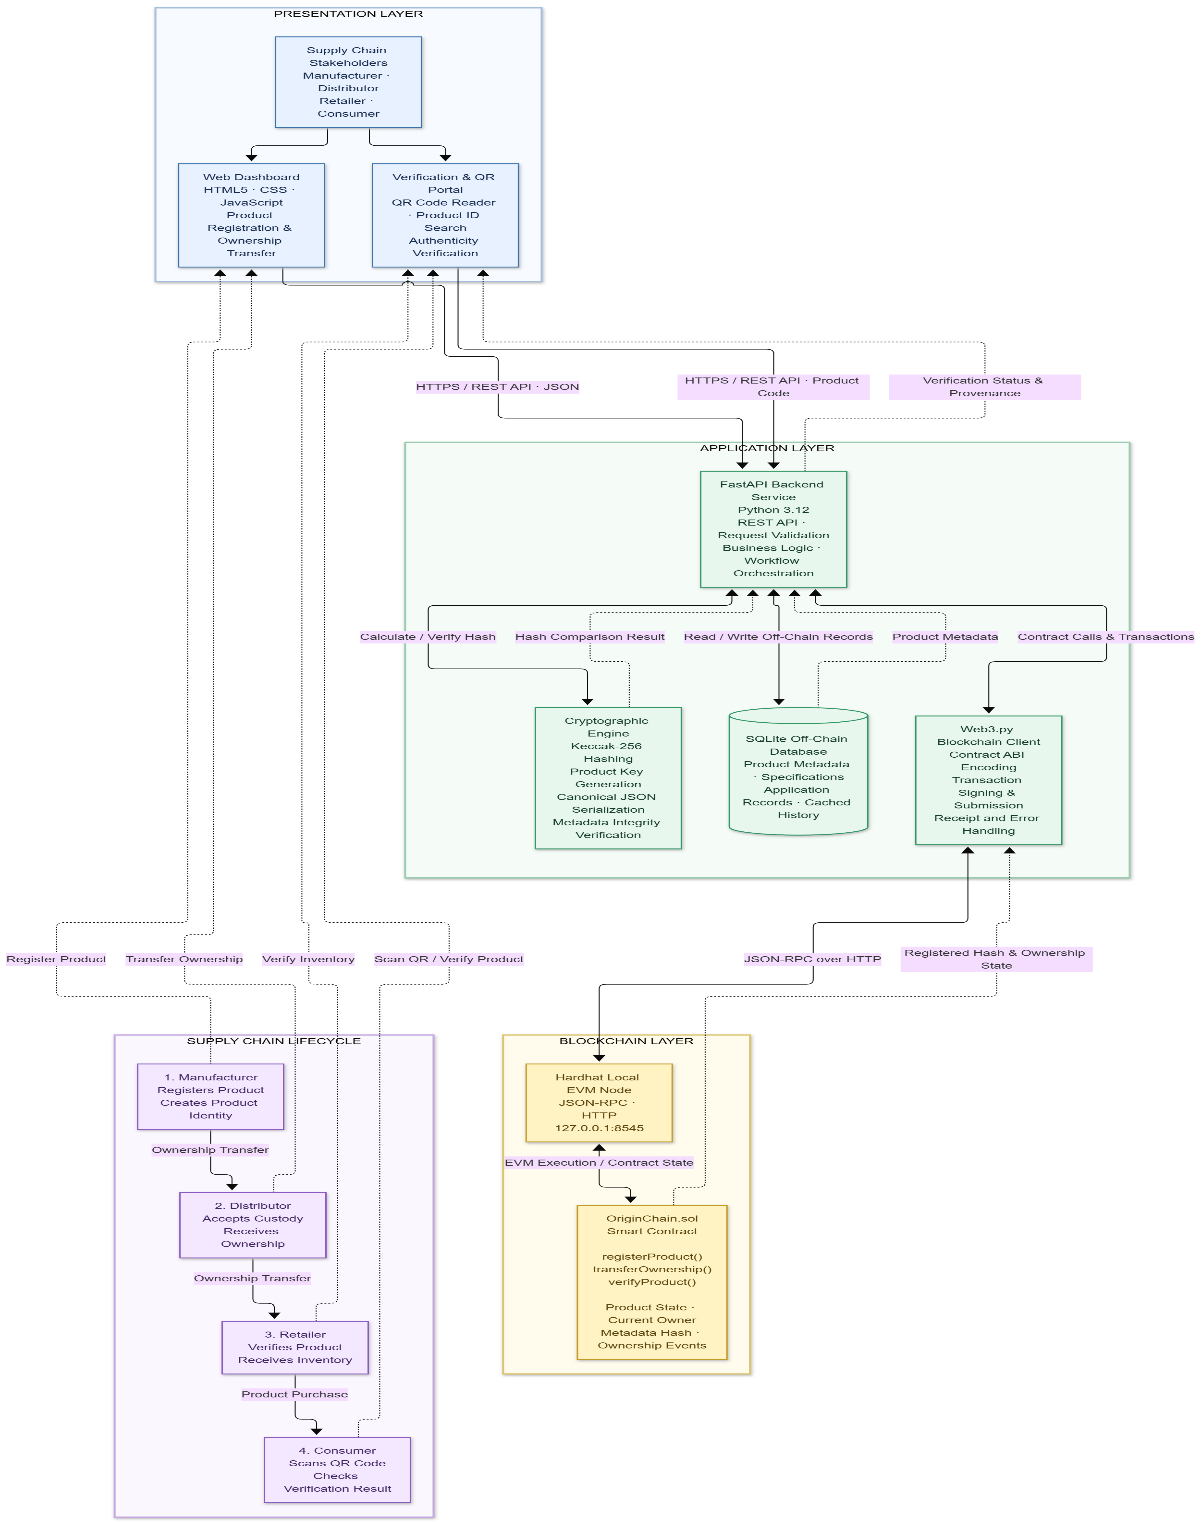
\includegraphics[width=0.82\textwidth,height=0.72\textheight,keepaspectratio]{images/fig_5_2_architecture.png}
\caption{Layered Architecture of OriginChain}
\label{fig:arch}
\end{figure}

\clearpage
\section{Use Case Diagram}
Figure 5.2 outlines the interactions between key supply-chain actors (Supplier, Manufacturer, Distributor, Retailer, Consumer, Admin) and the OriginChain platform.

\begin{figure}[H]
\centering
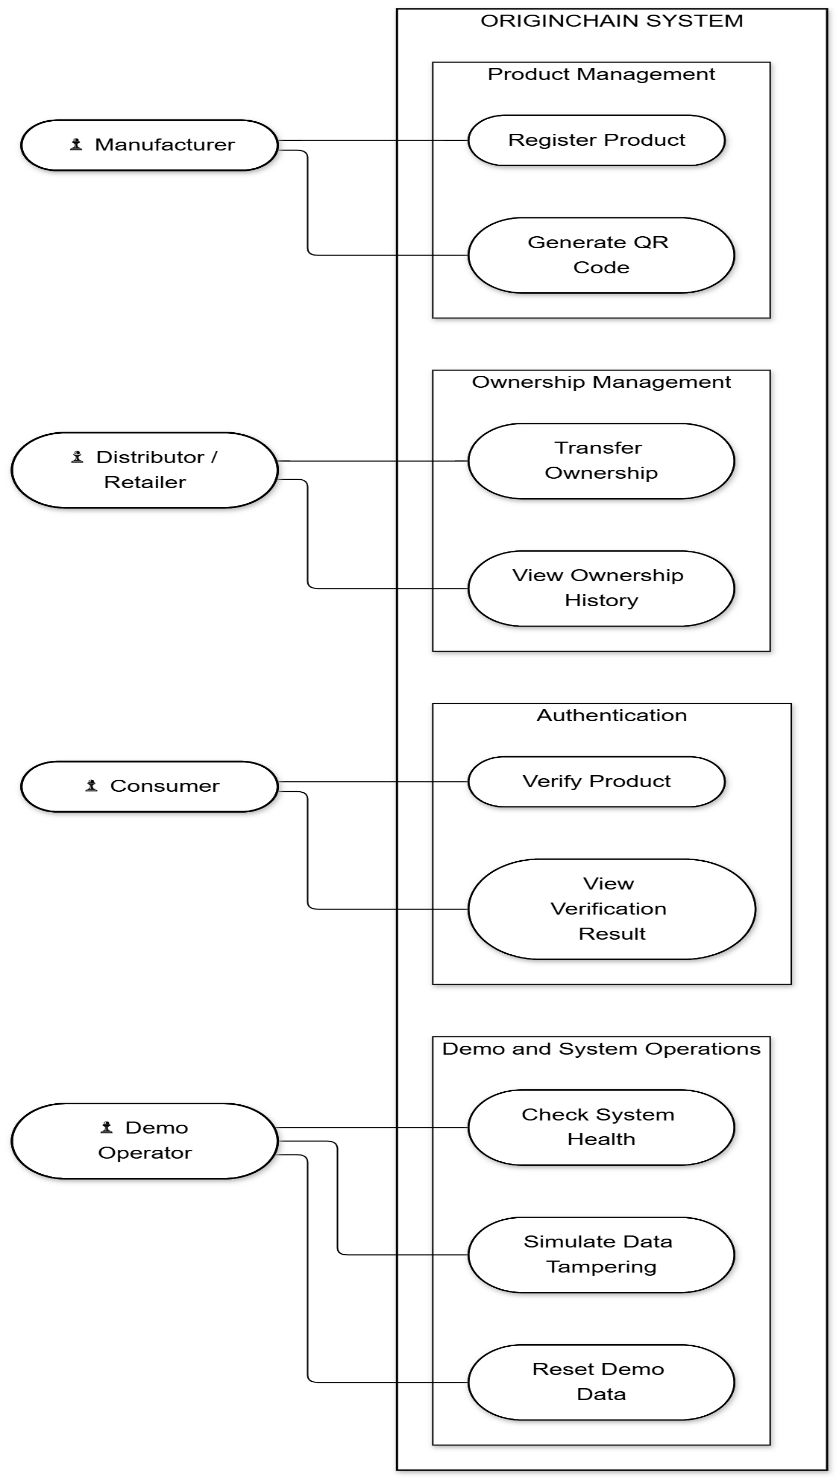
\includegraphics[width=0.80\textwidth,height=0.72\textheight,keepaspectratio]{images/fig_5_3_usecase.png}
\caption{Use Case Diagram of OriginChain}
\label{fig:usecase}
\end{figure}

\clearpage
\section{Workflow (Activity) Diagram}
Figure 5.3 shows the sequential workflow of a product from initial registration through stage quality evaluations, ownership transfers, and consumer QR verification.

\begin{figure}[H]
\centering
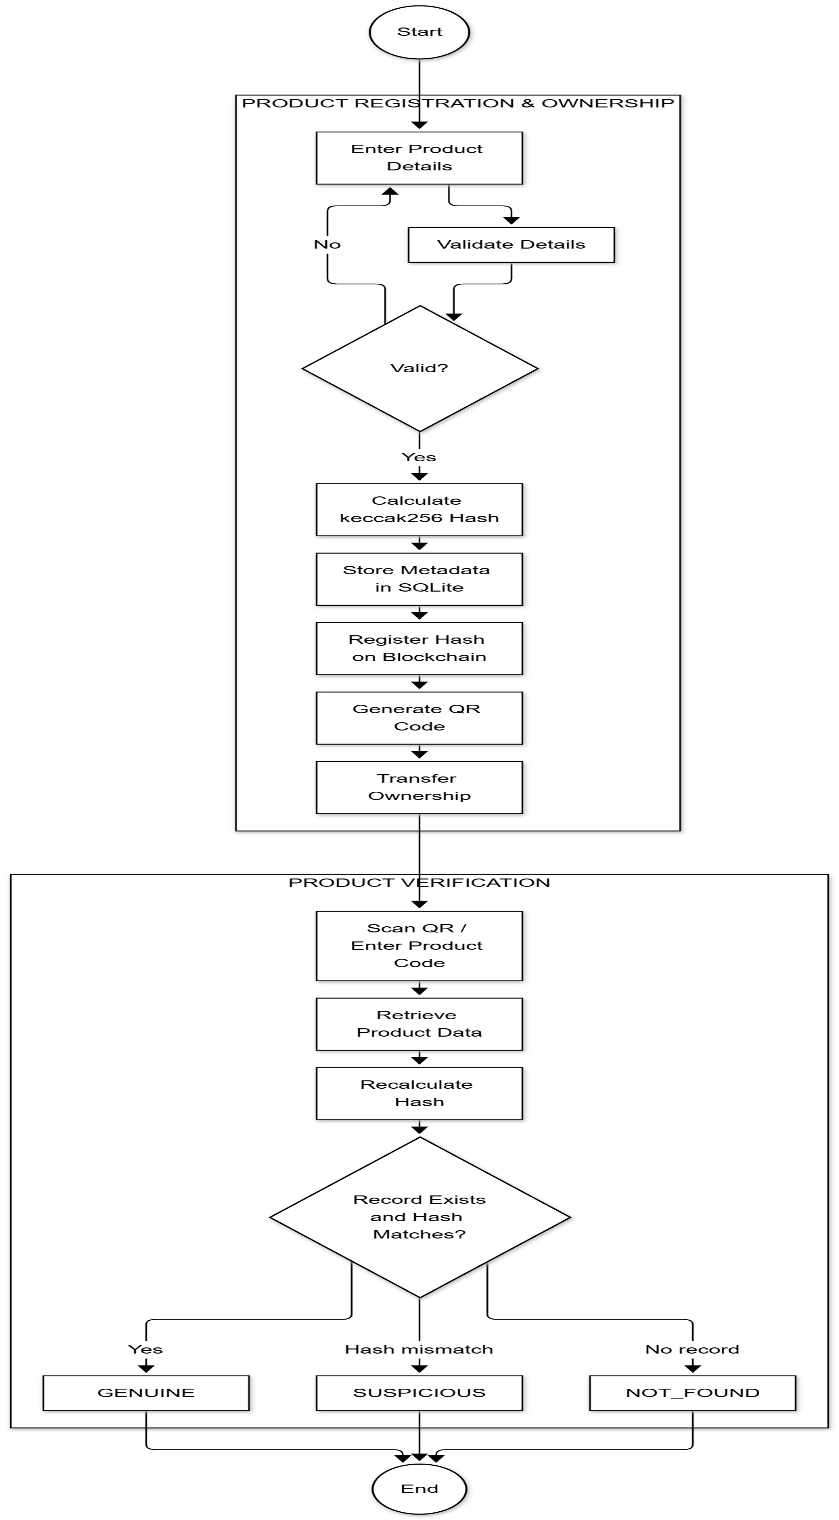
\includegraphics[width=0.80\textwidth,height=0.72\textheight,keepaspectratio]{images/fig_5_4_workflow.png}
\caption{End-to-End Workflow of a Product}
\label{fig:workflow}
\end{figure}

\clearpage
\section{Quality-Gate Flow}
Figure 5.4 depicts the decision logic executed during quality-gate evaluation for any operational stage.

\begin{figure}[H]
\centering
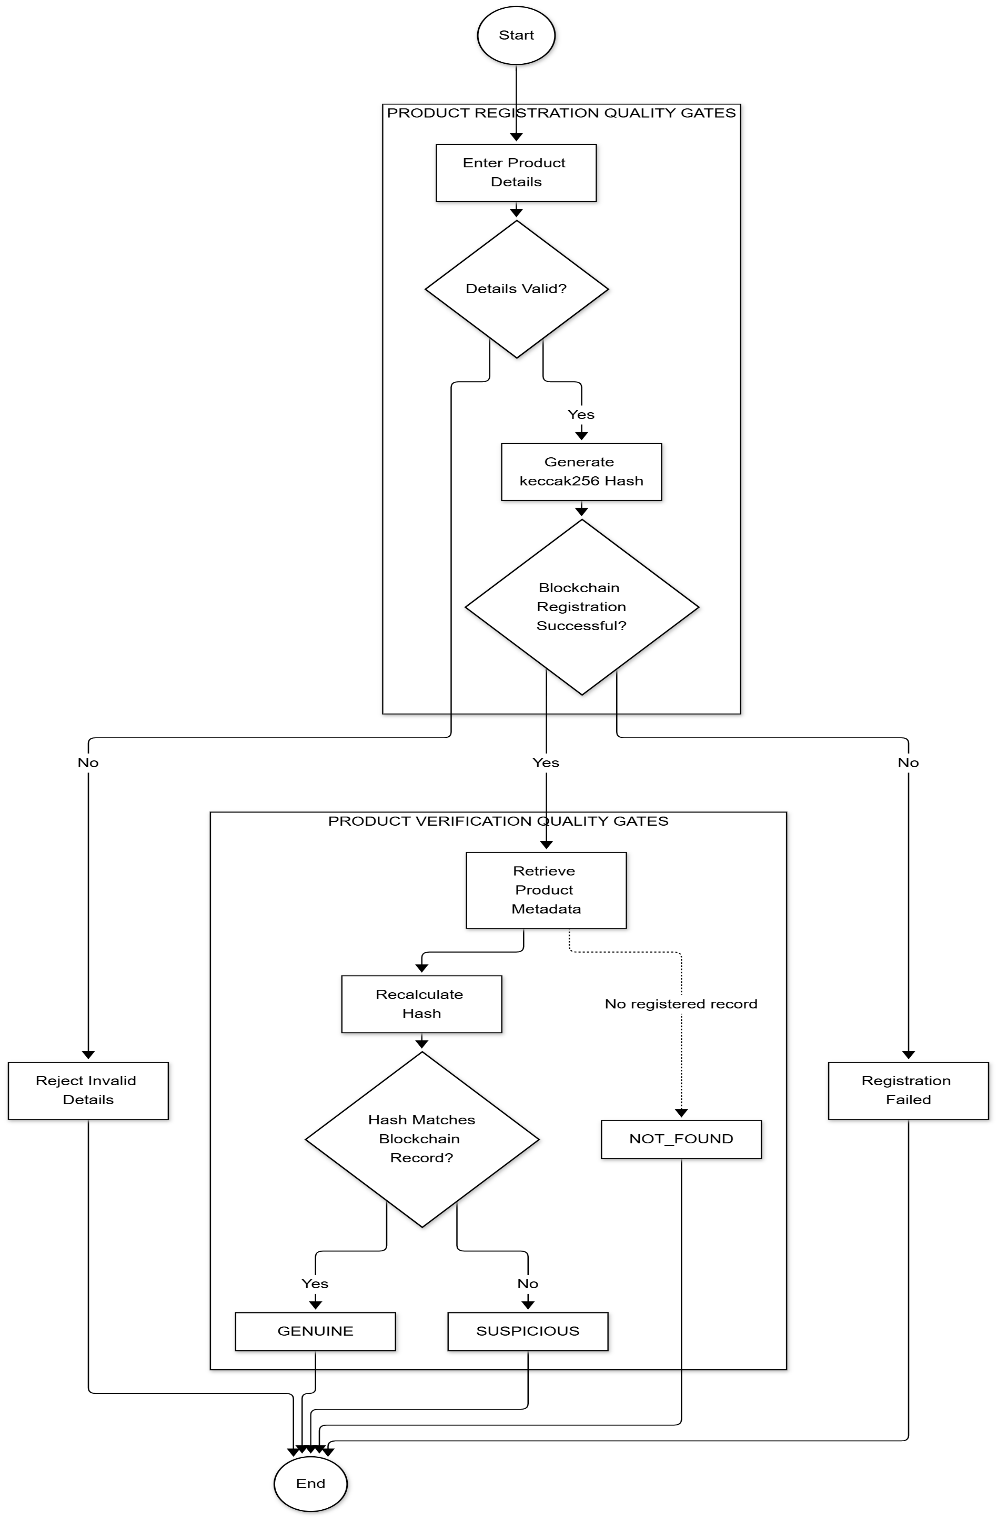
\includegraphics[width=0.82\textwidth,height=0.72\textheight,keepaspectratio]{images/fig_5_5_qualitygate.png}
\caption{Quality-Gate Evaluation for One Stage}
\label{fig:qualitygate}
\end{figure}

\clearpage
\section{Sequence Diagram}
Figure 5.5 illustrates the sequence of interactions between the user interface, FastAPI backend, SQLite database, and Solidity smart contract during product registration.

\begin{figure}[H]
\centering
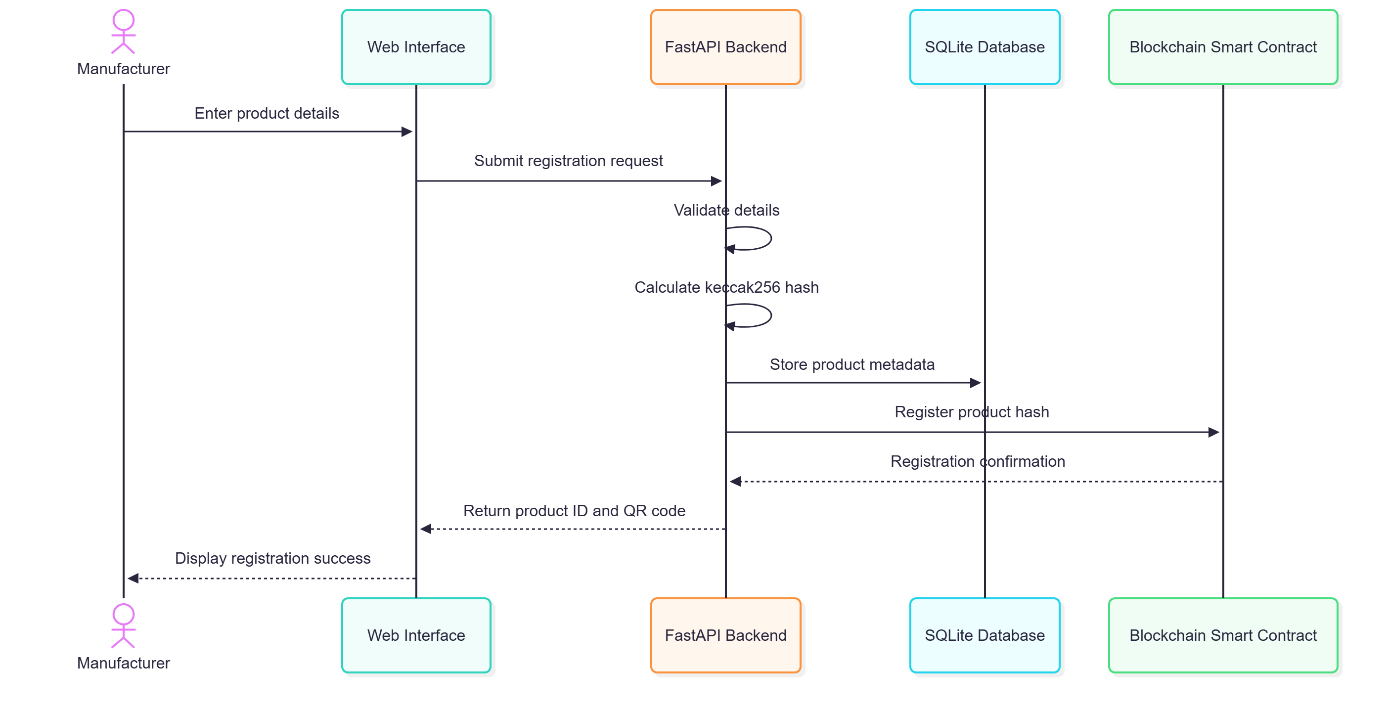
\includegraphics[width=0.98\textwidth,keepaspectratio]{images/fig_5_6_sequence.png}
\caption{Sequence Diagram for Product Registration}
\label{fig:sequence}
\end{figure}

\clearpage
\section{Class Diagram of the Smart Contract}
Figure 5.6 presents the class structure of the \texttt{OriginChain} smart contract, including structs, state mappings, function signatures, and events.

\begin{figure}[H]
\centering
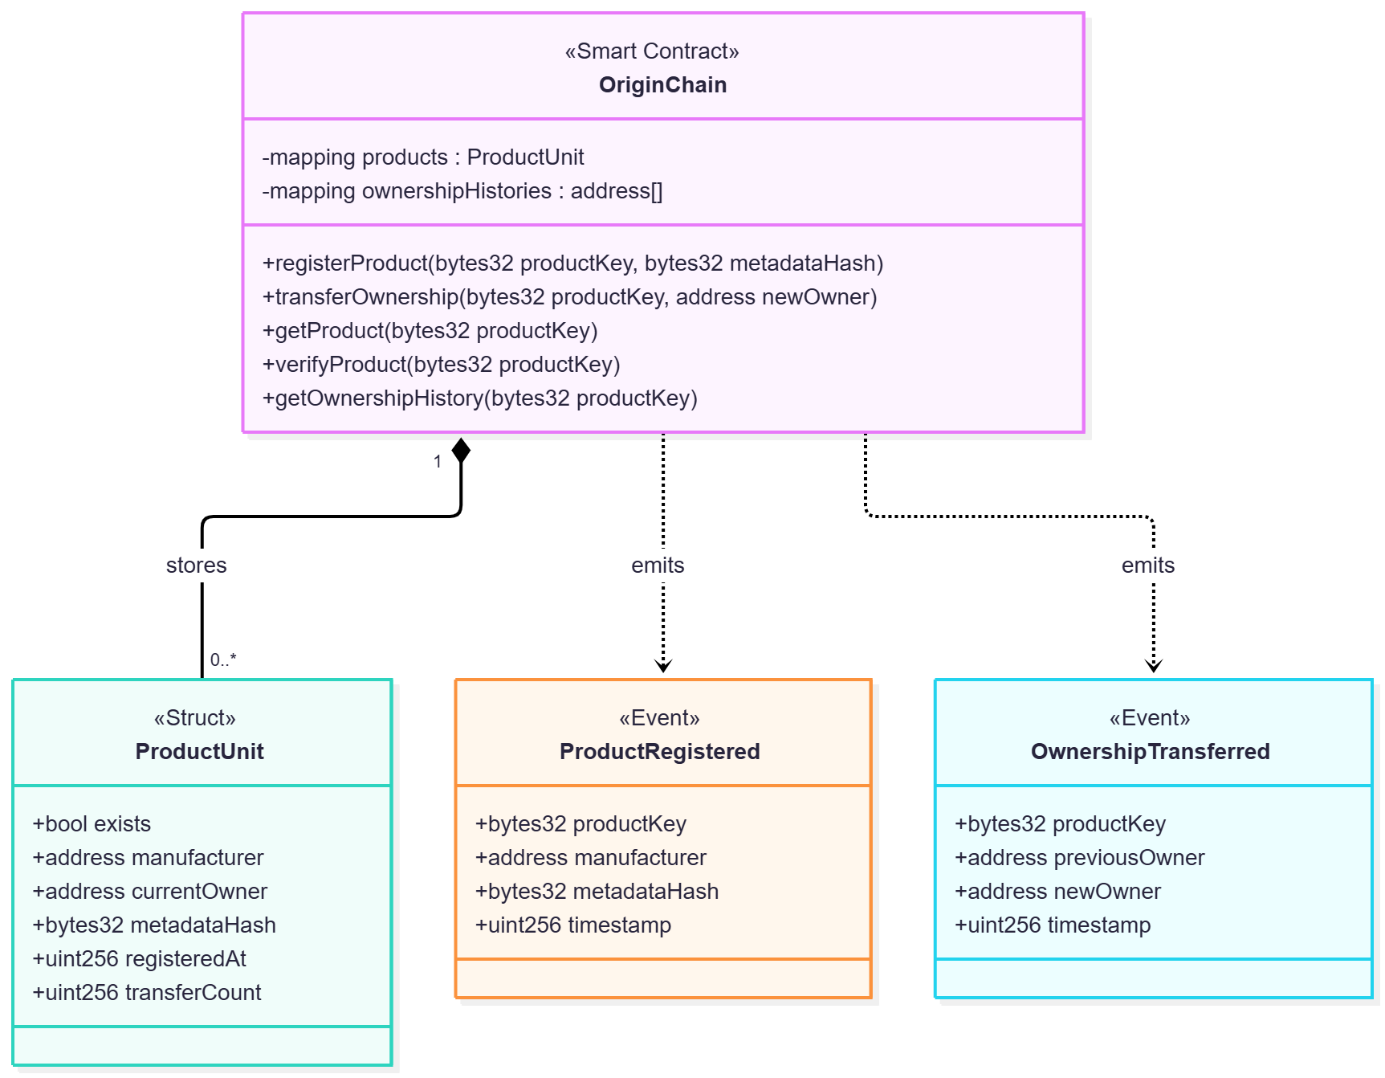
\includegraphics[width=0.95\textwidth,height=0.72\textheight,keepaspectratio]{images/fig_5_7_classdiagram.png}
\caption{Class Diagram of the OriginChain Smart Contract}
\label{fig:classdiagram}
\end{figure}

\clearpage
\section{Entity-Relationship Diagram}
Figure 5.7 shows the relational database schema implemented in SQLite, modeling users, products, batches, stages, checks, and evidence records.

\begin{figure}[H]
\centering
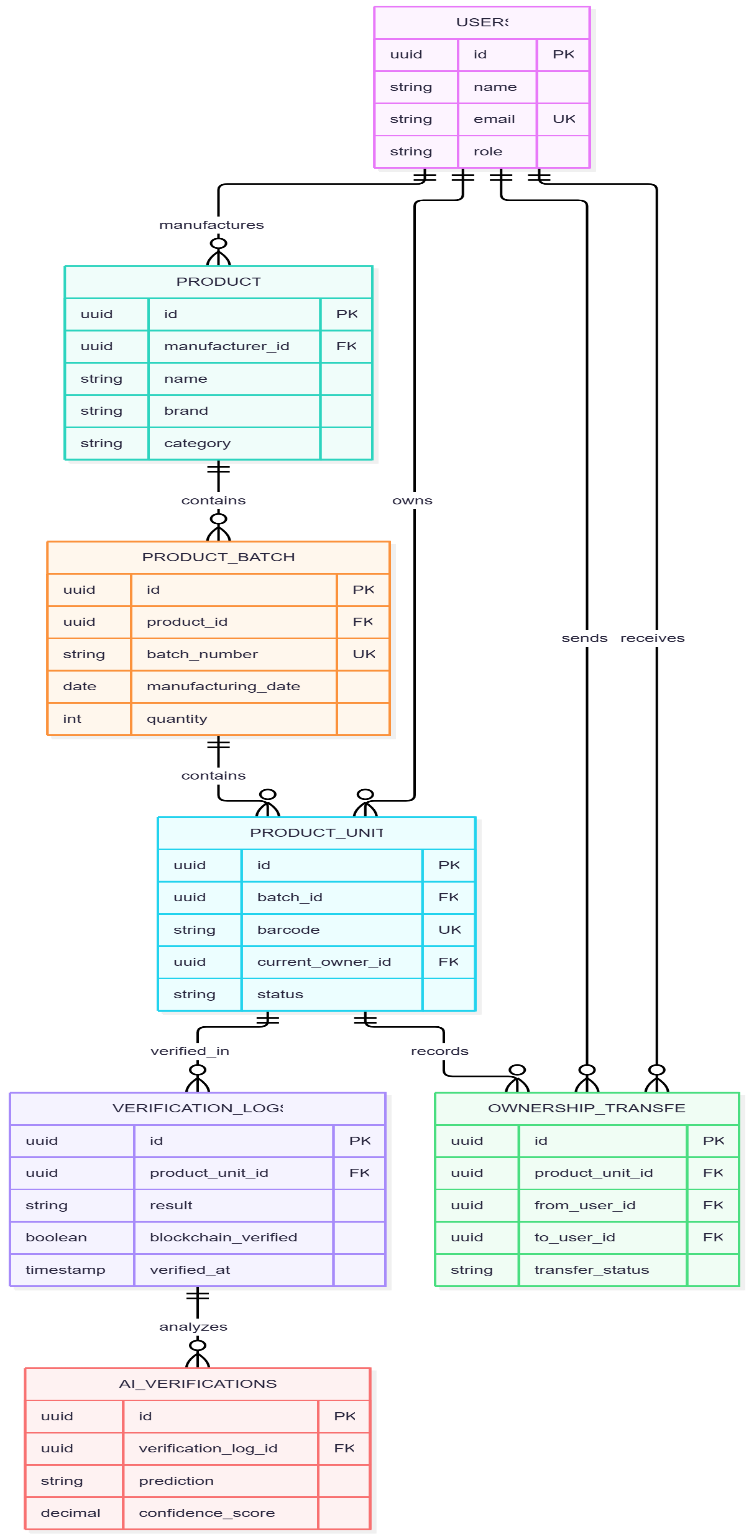
\includegraphics[width=0.75\textwidth,height=0.72\textheight,keepaspectratio]{images/fig_5_8_erd.png}
\caption{Entity-Relationship Diagram (Core SQLite Entities)}
\label{fig:erd}
\end{figure}

\clearpage
\section{Algorithms}
\noindent \textbf{Algorithm 1: Product Metadata Hashing}
\begin{enumerate}[leftmargin=1.8em, itemsep=3pt, parsep=0pt]
    \item Build a metadata dictionary with canonical keys: \texttt{batch\allowbreak\_number}, \texttt{brand}, \texttt{description}, \texttt{name}, and \texttt{product\allowbreak\_code}.
    \item Serialize into canonical JSON with sorted keys, no whitespace padding, and UTF-8 encoding.
    \item Compute the metadata hash:
    \[
    H = \text{Keccak-256}(\text{canonical\_JSON})
    \]
    \item Compute the product key:
    \[
    K = \text{Keccak-256}(\text{trimmed}(\text{product\_code}))
    \]
    \item Invoke \texttt{registerProduct(K, H)} on the smart contract; record $K$, $H$, and the transaction hash in SQLite.
\end{enumerate}

\vspace{0.4cm}
\noindent \textbf{Algorithm 2: Stage Approval Logic}
\begin{enumerate}[leftmargin=1.8em, itemsep=3pt, parsep=0pt]
    \item Retrieve all mandatory and optional checks for the active stage.
    \item If any mandatory check has failed, transition the stage status to \texttt{HOLD}; if any mandatory check is incomplete, maintain status as \texttt{PENDING}.
    \item For checks requiring documentation, verify that the uploaded evidence file exists and that its live byte hash matches the recorded hash.
    \item Verify that critical reports originate from an issuer recognized as \texttt{TRUSTED\_DEMO} in the trust registry.
    \item If all checks pass, build the stage snapshot, commit the snapshot hash and evidence hashes to the smart contract, and transition the stage status to \texttt{APPROVED}.
\end{enumerate}

\vspace{0.4cm}
\noindent \textbf{Algorithm 3: Consumer Verification}
\begin{enumerate}[leftmargin=1.8em, itemsep=3pt, parsep=0pt]
    \item Search the product in the local repository by \texttt{product\_code}; if absent, return \texttt{NOT\_FOUND}.
    \item Recompute canonical metadata hash $H_{\text{local}}$ from SQLite records and query on-chain commitment $H_{\text{chain}}$ from the smart contract.
    \item If $H_{\text{local}} \neq H_{\text{chain}}$, return \texttt{SUSPICIOUS} with a tamper alert flag.
    \item Otherwise, return \texttt{AUTHENTIC} with the redacted stage timeline, role-based provenance, and public evidence attachments.
\end{enumerate}

\clearpage
\section{Design Details}
\begin{table}[H]
\centering
\caption{Backend Modules and Responsibilities}
\label{tab:modules}
\small
\renewcommand{\arraystretch}{1.22}
\begin{tabularx}{\textwidth}{L{4.2cm} Y}
\toprule
\textbf{Module} & \textbf{Responsibility} \\
\midrule
\texttt{main.py} & FastAPI application routes for auth, records, quality, evidence, transfers, and demo \\
\texttt{database.py} & SQLite schema (20 tables), query repositories, and immutability guards \\
\texttt{domain.py} & Core domain entities, stage definitions, and seeded quality templates (24 checks) \\
\texttt{quality\_service.py} & Evaluation of stage gates, required checks, evidence integrity, and issuer trust \\
\texttt{auth.py} & Argon2 password hashing, 30-minute JWT creation, and per-request identity checks \\
\texttt{evidence.py} & File upload validation (PDF/PNG/JPEG, $\le 5$ MiB), safe path storage, and hashing \\
\texttt{metadata\_hash.py} & Canonical metadata serialization and Keccak-256 fingerprinting \\
\texttt{blockchain\_client.py} & Web3.py wrapper mapping supply-chain roles to server-held Ethereum signers \\
\texttt{presentation\_demo.py} & Automated scenario seeding and live interactive tampering demonstrations \\
\bottomrule
\end{tabularx}
\end{table}

\begin{table}[H]
\centering
\caption{Roles and Permitted Actions}
\label{tab:roles}
\small
\renewcommand{\arraystretch}{1.22}
\begin{tabularx}{\textwidth}{L{3.2cm} Y}
\toprule
\textbf{Role} & \textbf{Permitted Actions} \\
\midrule
Supplier & Register raw material batches; perform and approve raw-material quality checks \\
Manufacturer & Register finished products; complete manufacturing QC; transfer custody to Distributor \\
Distributor & Complete distribution storage and handling QC; transfer custody to Retailer \\
Retailer & Complete retail receiving QC; record final sale decision \\
Admin & View all stages, audit logs, and trust registries; trigger demo tampering scenarios \\
Consumer & Public read-only verification; no account required \\
\bottomrule
\end{tabularx}
\end{table}

\begin{table}[H]
\centering
\caption{Data Placement Matrix}
\label{tab:dataplc}
\small
\renewcommand{\arraystretch}{1.22}
\begin{tabularx}{\textwidth}{L{4.0cm} Y}
\toprule
\textbf{Location} & \textbf{Stored Information} \\
\midrule
On-Chain (Solidity) & Product key hash, metadata hash, current owner address, stage status, commitment snapshot hashes, evidence hashes, and transfer events \\
SQLite Database & User credentials (Argon2), audit trails, detailed product records, quality check results, specifications, issuer registries, and transaction receipts \\
File System & Raw uploaded evidence files under \texttt{backend/uploads/}, indexed by random UUIDs \\
\bottomrule
\end{tabularx}
\end{table}

\section{Methodology}
The project followed an agile, test-driven engineering approach. Core smart contract constraints were authored and verified first in Hardhat, followed by backend REST endpoints in FastAPI. The quality gate engine was integrated with deterministic seeding, followed by evidence file hashing and role-based access enforcement. Finally, the responsive web interface was integrated and validated using end-to-end automated smoke tests.

% -------------------------------------------------------------
% CHAPTER 6: EXPERIMENTAL SETUP
% -------------------------------------------------------------
\chapter{Experimental Setup}

\section{Database and Input Data}
The platform operates on a local SQLite database populated with deterministic test data, summarized in Table 6.1.

\begin{table}[H]
\centering
\caption{Seeded Input Data of the Demonstration}
\label{tab:seed_data}
\small
\renewcommand{\arraystretch}{1.22}
\begin{tabularx}{\textwidth}{L{4.2cm} Y}
\toprule
\textbf{Item} & \textbf{Details} \\
\midrule
Operational Users & 5 accounts (Supplier, Manufacturer, Distributor, Retailer, Admin) with Argon2 passwords \\
Flagship Product & Aurelia Prestige Renewal Serum, Code: \texttt{OC\allowbreak-LUX\allowbreak-SERUM\allowbreak-0001}, Batch: \texttt{APR\allowbreak-2026\allowbreak-001} \\
Quality Templates & 24 checks: 5 Supplier, 8 Manufacturer, 5 Distributor, 6 Retail \\
Product Specification & 1 versioned specification covering 16 physical and chemical attributes \\
Evidence Issuers & 6 fictional testing laboratories with \texttt{TRUSTED\_DEMO}, \texttt{UNVERIFIED}, or \texttt{REVOKED} status \\
Standards Registry & Metadata for Indian Cosmetics Rules 2020, BIS standards, and ISO 22716, 17516, 11930, 29621 \\
Evidence Files & Realistic PDF, PNG, and JPEG documents ($\le 5$ MiB) uploaded at each stage \\
\bottomrule
\end{tabularx}
\end{table}

\section{Performance Evaluation Parameters}
System validation evaluates correctness, gate enforcement, and cryptographic integrity, as defined in Table 6.2.

\begin{table}[H]
\centering
\caption{Evaluation Parameters Used for Validation}
\label{tab:eval_params}
\small
\renewcommand{\arraystretch}{1.20}
\begin{tabularx}{\textwidth}{L{4.2cm} Y}
\toprule
\textbf{Parameter} & \textbf{How It Is Validated} \\
\midrule
Functional Correctness & End-to-end traversal from raw materials to final sale approval \\
Gate Enforcement & Custody transfers strictly blocked while mandatory checks or evidence are missing \\
Tamper Detection & Modifying SQLite records immediately triggers \texttt{SUSPICIOUS} during consumer verification \\
Evidence Integrity & Cryptographic re-hashing flags \texttt{VERIFIED}, \texttt{MISMATCH}, or \texttt{FILE\_MISSING} \\
Issuer Trust Handling & Revoked issuers cannot authorize critical evidence; historical approvals remain frozen \\
Access Control & Server-side RBAC and contract-level caller validation reject unauthorized operations \\
Consumer Privacy & Internal notes, internal identifiers, and private files are stripped from consumer responses \\
Smart Contract Safety & Duplicate registrations and transfers by non-owners are rejected by EVM reverts \\
Test Suite Pass Rate & 100\% pass rate across 51 backend unit/integration tests and 17 smart contract tests \\
\bottomrule
\end{tabularx}
\end{table}

\clearpage
\noindent Figure 6.1 shows the distribution of automated test suites covering the application.

\begin{figure}[H]
\centering
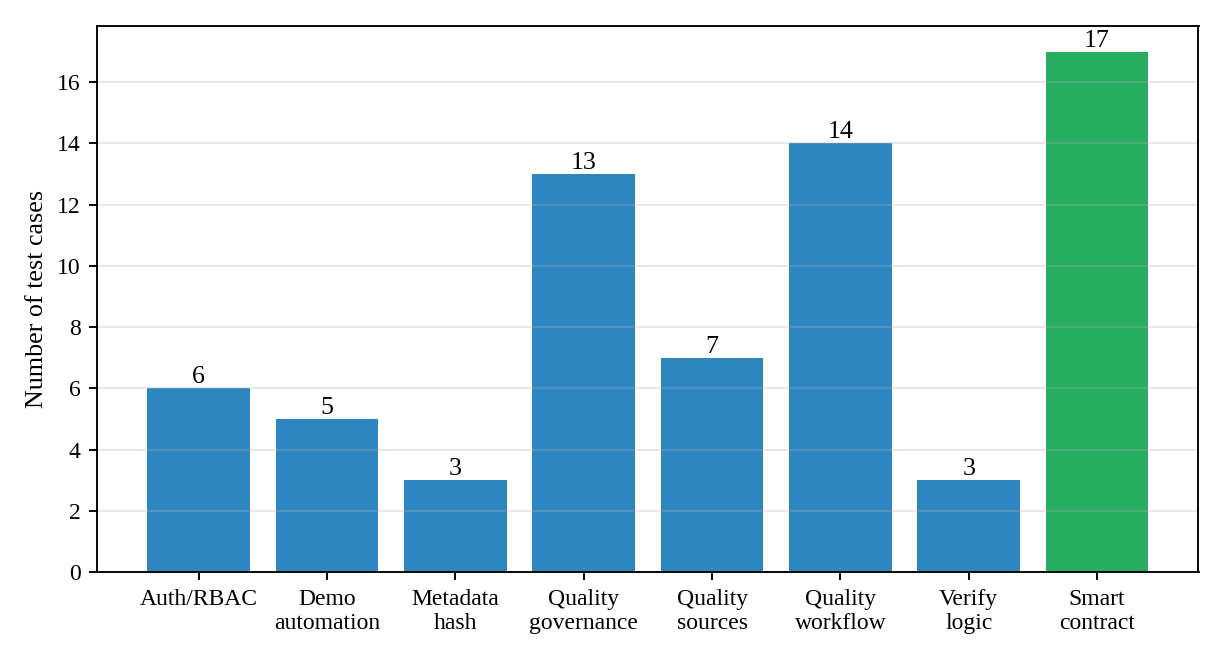
\includegraphics[width=0.85\textwidth,keepaspectratio]{images/graph_6_1_testcases.png}
\caption{Automated Test Cases per Suite (68 Total Tests)}
\label{fig:tests}
\end{figure}

\section{Software and Hardware Setup}
Tables 6.3 and 6.4 list the software tools and minimum hardware specifications required to run OriginChain.

\begin{table}[H]
\centering
\caption{Software Requirements}
\label{tab:sw_req}
\small
\renewcommand{\arraystretch}{1.22}
\begin{tabularx}{\textwidth}{L{4.0cm} Y}
\toprule
\textbf{Component} & \textbf{Version / Tool} \\
\midrule
Operating System & Linux (Ubuntu 22.04+), macOS, or Windows 10/11 \\
Backend Framework & Python 3.13, FastAPI 0.116+, Uvicorn, Web3.py 8, PyJWT, Argon2, QRCode \\
Blockchain Environment & Node.js 22.13+, Hardhat 3.15, Ethers.js 6, Solidity 0.8.28+ \\
Database & SQLite 3 \\
Frontend & HTML5, CSS3, Vanilla JavaScript (ES6+) \\
Testing Framework & Pytest 9, Hardhat Test Runner, Headless Chrome \\
\bottomrule
\end{tabularx}
\end{table}

\begin{table}[H]
\centering
\caption{Hardware Requirements}
\label{tab:hw_req}
\small
\renewcommand{\arraystretch}{1.22}
\begin{tabularx}{\textwidth}{L{4.0cm} Y}
\toprule
\textbf{Item} & \textbf{Specification} \\
\midrule
Processor & Modern dual-core CPU (2.0 GHz or higher) \\
RAM & 8 GB recommended (minimum 4 GB) \\
Storage & 1 GB available disk space for dependencies, database, and uploads \\
Network & No external internet connection required; runs entirely on localhost \\
\bottomrule
\end{tabularx}
\end{table}

% -------------------------------------------------------------
% CHAPTER 7: PROJECT PLAN
% -------------------------------------------------------------
\chapter{Project Plan}

\section{Gantt Chart}
The project timeline spans literature review, smart contract development, backend implementation, quality gate engine, frontend interface, and validation, as shown in Figure 7.1.

\begin{figure}[H]
\centering
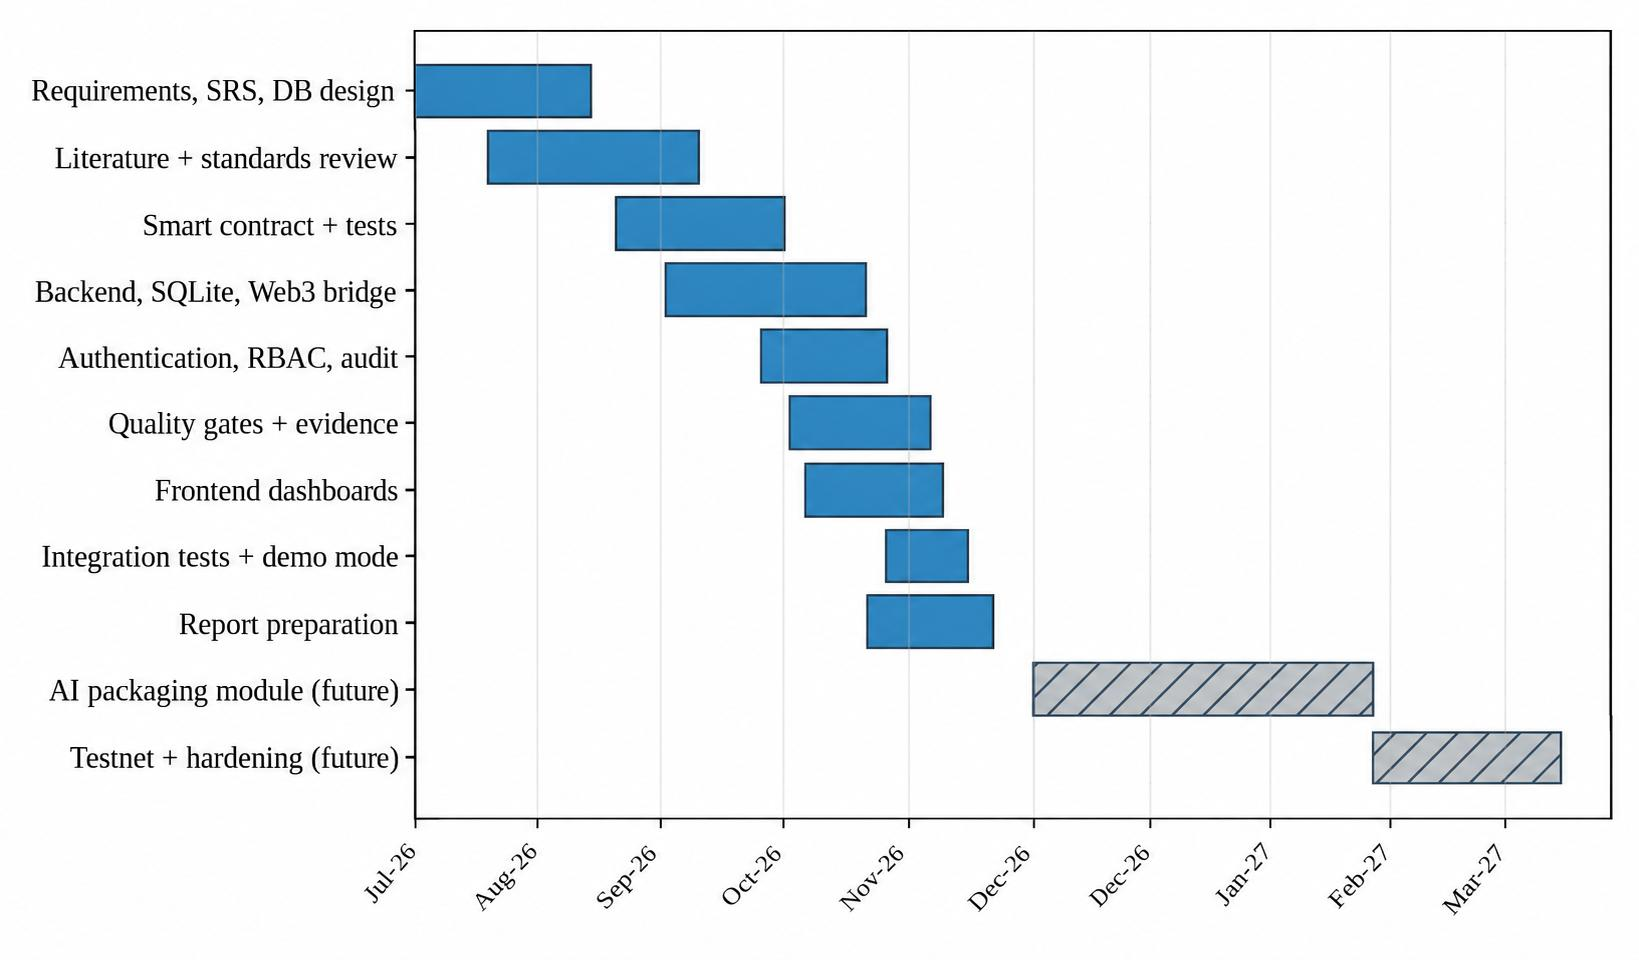
\includegraphics[width=\textwidth,keepaspectratio]{images/fig_7_1_gantt.png}
\caption{Gantt Chart of the Project Plan}
\label{fig:gantt}
\end{figure}

\section{Team and Responsibilities}
Table 7.1 outlines the division of responsibilities among the four project team members.

\begin{table}[H]
\centering
\caption{Team Roles and Responsibilities}
\label{tab:team_roles}
\small
\renewcommand{\arraystretch}{1.22}
\begin{tabularx}{\textwidth}{L{4.2cm} L{3.8cm} Y}
\toprule
\textbf{Member} & \textbf{Role} & \textbf{Key Responsibilities} \\
\midrule
Durva Waghchaure & Backend \& Project Lead & FastAPI architecture, quality gates, authentication, and report compilation \\
Aradhya Thakur & Frontend Lead & Single-page interface, responsive styling, and QR verification UX \\
Aryan Singh & Blockchain Lead & Solidity smart contract, Hardhat test suites, and Web3 integration \\
Purvika Thombare & AI \& Quality Lead & Standards metadata registry, evidence verification, and AI packaging research \\
\bottomrule
\end{tabularx}
\end{table}

Phases progressed from initial requirements capture and standards mapping to smart contract deployment, backend API implementation, quality gating, frontend UI assembly, and documentation preparation.

% -------------------------------------------------------------
% CHAPTER 8: EXPECTED OUTCOME
% -------------------------------------------------------------
\chapter{Expected Outcome}

The implementation of OriginChain delivers the following tangible results:

\begin{enumerate}[leftmargin=1.8em, itemsep=4pt, parsep=0pt]
    \item \textbf{Working End-to-End Traceability System:} A functional application demonstrating custody and quality hand-offs for luxury cosmetics from ingredient supplier to retail sale.
    \item \textbf{Tamper-Evident Product Identity:} Any unauthorized alteration of product records in the application database is instantly flagged as \texttt{SUSPICIOUS} during consumer verification.
    \item \textbf{Cryptographically Verifiable Evidence:} All certificates and inspection documents are bound to Keccak-256 hashes, with on-demand status reporting (\texttt{VERIFIED}, \texttt{MISMATCH}, or \texttt{FILE\_MISSING}).
    \item \textbf{Attributable Audit Logging:} All operational events are logged with authenticated user identities, timestamps, and stage tags in an admin audit trail.
    \item \textbf{Dual-Tier Access Control:} Enforcement of stage-specific business rules in FastAPI and cryptographic caller verification in Solidity smart contracts.
    \item \textbf{Privacy-Preserving Consumer Portal:} Read-only consumer verification displaying authenticity status and provenance milestones without leaking proprietary commercial information.
    \item \textbf{Standards-Aligned Quality Architecture:} Clear mapping of quality checks to Indian Cosmetics Rules 2020 and ISO standards metadata.
    \item \textbf{Automated Test Suite:} Complete test coverage comprising 51 backend tests and 17 smart contract tests ensuring robustness and reproducibility.
\end{enumerate}

% -------------------------------------------------------------
% CHAPTER 9: PROJECTED COST ANALYSIS
% -------------------------------------------------------------
\chapter{Projected Cost Analysis}

Because OriginChain operates entirely on open-source software and a local EVM test network, development and demonstration costs are zero. Table 9.1 provides an indicative cost breakdown for prototyping and potential production deployment.

\begin{table}[H]
\centering
\caption{Projected Cost Analysis (Indicative Estimates)}
\label{tab:cost}
\small
\renewcommand{\arraystretch}{1.22}
\begin{tabularx}{\textwidth}{L{4.5cm} L{4.5cm} Y}
\toprule
\textbf{Component} & \textbf{Technology Used} & \textbf{Estimated Prototype Cost (INR)} \\
\midrule
Smart Contract \& EVM & Solidity, Hardhat & \textbf{INR 0} \\
Backend API & Python, FastAPI, Web3.py & \textbf{INR 0} \\
Database \& Evidence Storage & SQLite, Local File System & \textbf{INR 0} \\
Frontend Interface & HTML5, CSS3, Vanilla JavaScript & \textbf{INR 0} \\
Blockchain Gas Fees & Hardhat Local Test ETH & \textbf{INR 0} \\
Hosting Infrastructure & Local Developer Laptop & \textbf{INR 0} \\
\midrule
\textbf{Total Prototype Cost} & & \textbf{INR 0} \\
\bottomrule
\end{tabularx}
\end{table}

\noindent \textbf{Production Cost Projection:}
In production deployment, blockchain transaction costs depend heavily on the target network. OriginChain requires 14 on-chain transactions per product batch across all four supply-chain stages. On the Polygon proof-of-stake network, this translates to approximately INR~2.50 ($\approx \$0.03$) per batch, compared to upwards of INR~2,000 on Ethereum mainnet. A hosted enterprise pilot managing 100 batches per month would incur approximately INR~1,200 ($\approx \$15$) monthly, primarily for cloud virtual machine hosting and database backups.

% -------------------------------------------------------------
% REFERENCES
% -------------------------------------------------------------
\begin{thebibliography}{99}
\addcontentsline{toc}{chapter}{References}
\small
\setlength{\itemsep}{1.5pt}
\setlength{\parsep}{0pt}

\bibitem{ref1} OECD and European Union Intellectual Property Office (EUIPO), \textit{Global Trade in Fakes: A Worrying Threat}, Paris, France: OECD Publishing, 2021. doi: 10.1787/74c81154-en.

\bibitem{ref2} S. Nakamoto, ``Bitcoin: A peer-to-peer electronic cash system,'' \textit{Decentralized Business Review}, 2008.

\bibitem{ref3} Z. Zheng, S. Xie, H. Dai, X. Chen, and H. Wang, ``An overview of blockchain technology: Architecture, consensus, and future trends,'' in \textit{Proc. IEEE Int. Congr. Big Data}, 2017, pp. 557--564.

\bibitem{ref4} G. Wood, ``Ethereum: A secure decentralised generalised transaction ledger,'' \textit{Ethereum Project Yellow Paper}, vol. 151, pp. 1--32, 2014.

\bibitem{ref5} K. Christidis and M. Devetsikiotis, ``Blockchains and smart contracts for the Internet of Things,'' \textit{IEEE Access}, vol. 4, pp. 2292--2303, 2016.

\bibitem{ref6} Q. Lu and X. Xu, ``Adaptable blockchain-based systems: A case study for product traceability,'' \textit{IEEE Software}, vol. 34, no. 6, pp. 21--27, 2017.

\bibitem{ref7} Ministry of Health and Family Welfare, Government of India, \textit{Cosmetics Rules, 2020}, Gazette of India, Extraordinary, Part II, Section 3, Sub-section (i), Nov. 2020.

\bibitem{ref8} International Organization for Standardization, \textit{Cosmetics --- Good Manufacturing Practices (GMP) --- Guidelines on Good Manufacturing Practices}, ISO 22716:2007, 2007.

\bibitem{ref9} International Organization for Standardization, \textit{Cosmetics --- Microbiology --- Microbiological limits}, ISO 17516:2014, 2014.

\bibitem{ref10} International Organization for Standardization, \textit{Cosmetics --- Microbiology --- Guidelines for the risk assessment and identification of microbiologically low-risk products}, ISO 29621:2017, 2017.

\bibitem{ref11} International Organization for Standardization, \textit{Cosmetics --- Microbiology --- Evaluation of the antimicrobial protection of a cosmetic product}, ISO 11930:2019, 2019.

\bibitem{ref12} A. Biryukov, D. Dinu, and D. Khovratovich, ``Argon2: New generation of memory-hard functions for password hashing and other applications,'' in \textit{Proc. IEEE European Symp. Security and Privacy (EuroS\&P)}, 2016, pp. 292--302.

\bibitem{ref13} M. Jones, J. Bradley, and N. Sakimura, ``JSON Web Token (JWT),'' RFC 7519, Internet Engineering Task Force (IETF), 2015.

\bibitem{ref14} Z. Zheng, S. Xie, H. Dai, X. Chen, and H. Wang, ``Blockchain challenges and opportunities: A survey,'' \textit{Int. J. Web and Grid Services}, vol. 14, no. 4, pp. 352--375, 2018.

\bibitem{ref15} A. Reyna, C. Martín, J. Chen, E. Soler, and M. Díaz, ``On blockchain and its integration with IoT. Challenges and opportunities,'' \textit{Future Generation Computer Systems}, vol. 88, pp. 173--190, 2018.

\bibitem{ref16} F. Tian, ``An agri-food supply chain traceability system for China based on RFID \& blockchain technology,'' in \textit{Proc. 13th Int. Conf. Service Systems and Service Management (ICSSSM)}, 2016, pp. 1--6.

\bibitem{ref17} S. Saberi, M. Kouhizadeh, J. Sarkis, and L. Shen, ``Blockchain technology and its relationships to sustainable supply chain management,'' \textit{Int. J. Production Research}, vol. 57, no. 7, pp. 2117--2135, 2019.

\bibitem{ref18} M. Pournader, Y. Shi, S. Seuring, and S. C. L. Koh, ``Blockchain applications in supply chains, transport and logistics: A systematic review of the literature,'' \textit{Int. J. Production Research}, vol. 58, no. 7, pp. 2063--2081, 2020.

\bibitem{ref19} J. Sunny, N. Undralla, and V. M. Pillai, ``Supply chain transparency through blockchain-based traceability: An overview with demonstration,'' \textit{Computers \& Industrial Engineering}, vol. 150, p. 106895, 2020.

\bibitem{ref20} M. Westerkamp, F. Victor, and A. Küpper, ``Tracing manufacturing processes using blockchain-based token compositions,'' in \textit{Proc. IEEE Int. Conf. Blockchain and Cryptocurrency (ICBC)}, 2019, pp. 167--174.

\bibitem{ref21} K. Toyoda, P. T. Mathiopoulos, I. Sasase, and T. Ohtsuki, ``A novel blockchain-based product ownership management system (POMS) for anti-counterfeits in the post supply chain,'' \textit{IEEE Access}, vol. 5, pp. 17465--17477, 2017.

\bibitem{ref22} S. Alzahrani and N. Bulusu, ``Block-supply chain: A new anti-counterfeiting supply chain using NFC and blockchain,'' in \textit{Proc. 1st Workshop on Cryptocurrencies and Blockchains for Distributed Systems (CryBlock)}, 2018, pp. 30--35.

\bibitem{ref23} A. Kamilaris, A. Fonts, and F. X. Prenafeta-Boldú, ``The rise of blockchain technology in agriculture and food supply chains,'' \textit{Trends in Food Science \& Technology}, vol. 91, pp. 640--652, 2019.

\bibitem{ref24} T. Bocek, B. B. Rodrigues, T. Strasser, and B. Stiller, ``Blockchains everywhere --- A use-case of blockchains in the pharma supply-chain,'' in \textit{Proc. IFIP/IEEE Symp. Integrated Network and Service Management (IM)}, 2017, pp. 772--777.

\end{thebibliography}

\end{document}
